\section{Wavelet Thresholding Algorithm}

We use the Discrete Wavelet Transform (DWT) algorithm implementation in the \texttt{dwt()} function from the \pkg{wavselim} \proglang{R} package.
Our thresholding approach is as follows.

\begin{steps}
  \item \underline{Pad the Data to Ensure Dyadic Length}: The DWT can only be applied to vectors of dyadic length, i.e., a power of $2$.
  \begin{figure}[H]
      \centering
      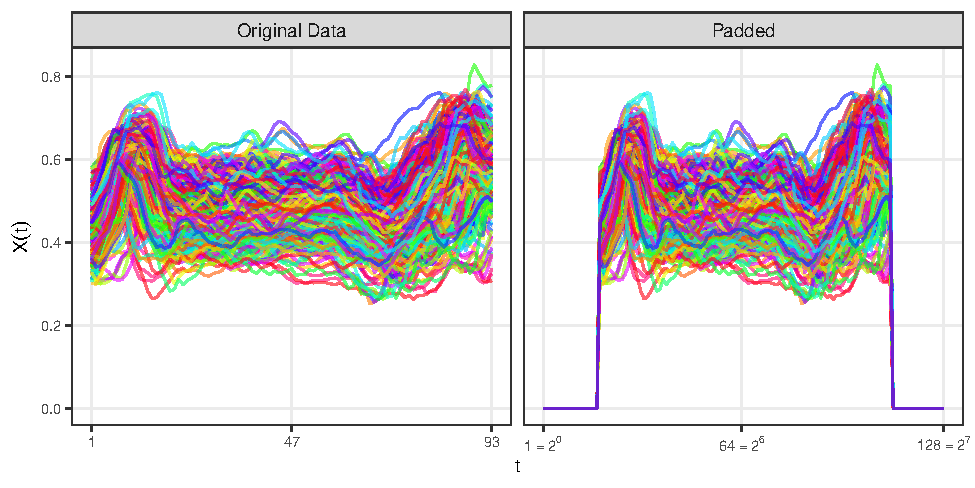
\includegraphics[width=0.5\linewidth]{figures/DTI-padded.pdf}
      \caption{Caption}
      \label{fig:enter-label}
  \end{figure}
  \item \underline{Apply the DWT to each Column of the Padded Data}:
  \item Third thing to do
\end{steps}
